\chapter{Teori Hückel dan Sistem Terkonjugasi}\label{ch:b2:huckel}

Tambahkan hidrogen pada sikloheksena, dan \qty{119}{kJ} dilepaskan per mol.
Benzena, dengan tiga ikatan rangkap dalam cincin enam karbon, seharusnya
melepaskan tiga kali lebih banyak dalam perjalanannya menjadi
sikloheksana; ternyata benzena melepaskan \qty{150}{kJ} lebih sedikit.
Energi yang hilang itu adalah kestabilan cincin \omterm{def:b2:huckel:aromatic}{aromatik}, alasan mengapa
benzena menolak reaksi-reaksi adisi yang dialami alkena. Pada tahun 1931
Erich Hückel menghitungnya dengan sebuah determinan, setelah menyederhanakan
molekul itu menjadi elektron-elektron $\pi$-nya dan tetangga-tetangganya.
Metodenya kasar, tetapi menjelaskan mengapa cincin dengan enam elektron
$\pi$ istimewa, mengapa rantai terkonjugasi yang panjang menyerap cahaya
tampak, dan di mana sebuah molekul terkonjugasi membawa muatan-muatannya.

\begin{recall}
\Cref{ch:b2:diatomic-mos}: \omterm{def:b2:diatomic-mos:integrals}{integral Coulomb} $\alpha$, \omterm{def:b2:diatomic-mos:integrals}{integral resonansi}
$\beta$, \omterm{def:b2:diatomic-mos:integrals}{determinan sekular}. \Cref{ch:b2:fragment-orbitals}: orbital $\pi$
etena dan alil. Jilid Tahun 1: sistem terkonjugasi, resonansi, kromofor,
dan maksimum serapan.
\end{recall}

\section{Metode Hückel}

Dalam molekul terkonjugasi yang datar, orbital-orbital $\sigma$ simetris
dan orbital-orbital p yang tegak lurus bidang antisimetris terhadap bidang
itu: keduanya tidak bercampur (\cref{prop:b2:diatomic-mos:symmetry}), dan
elektron-elektron $\pi$ dapat ditinjau tersendiri.

\begin{definition}[Metode Hückel]\label{def:b2:huckel:method}
Yang disebut \emph{metode Hückel}\index{metode Hückel} menghitung
orbital-orbital $\pi$ sistem terkonjugasi yang datar sebagai kombinasi
$\psi = \sum_r c_r p_r$ dari satu orbital p per atom, dengan
pendekatan-pendekatan: tumpang-tindih $S_{rs} = 0$ untuk $r \neq s$ (dan 1
untuk $r =
s$); semua \omterm{def:b2:diatomic-mos:integrals}{integral Coulomb} sama dengan $\alpha$; \omterm{def:b2:diatomic-mos:integrals}{integral
resonansi} sama dengan $\beta < 0$ di antara tetangga yang terikat dan nol
untuk yang lain.
\end{definition}

Dengan $x = (\alpha - E)/\beta$, persamaan-persamaan sekular menjadi, untuk
setiap atom $r$, $xc_r + \sum_{s \text{ terikat pada } r} c_s = 0$, dan
energi-energinya adalah akar-akar determinan dengan $x$ pada diagonal dan
1 di antara atom-atom yang terikat. Secara setara, $E =
\alpha + m\beta$
dengan $m$ nilai-nilai eigen matriks ketetanggaan kerangka karbon molekul
itu; karena $\beta < 0$, $m$ yang positif adalah tingkat ikatan.

\begin{method}[Perhitungan Hückel]\label{met:b2:huckel:huckel}
\begin{enumerate}
  \item Beri nomor atom-atom terkonjugasi; tuliskan matriks dengan 0 pada
        diagonal dan 1 untuk setiap pasangan yang terikat.
  \item Tentukan nilai-nilai eigennya $m_k$ (dengan bentuk tertutup di
        bawah, atau secara numerik): $E_k =
        \alpha + m_k\beta$.
  \item Isilah tingkat-tingkatnya mulai dari yang paling bersifat ikatan,
        dua elektron masing-masing: $E_\pi = \sum_k n_k E_k$.
  \item Dari koefisien-koefisien yang ternormalisasi, hitunglah muatan dan
        indeks ikatan.
\end{enumerate}
\end{method}

\begin{proposition}[Jejak matriks]\label{prop:b2:huckel:trace}
Energi $n$ orbital $\pi$ sebuah sistem Hückel berjumlah $n\alpha$.
\end{proposition}

\begin{proof}
Jumlah nilai-nilai eigen sebuah matriks adalah jejaknya (\textit{trace}); matriks Hückel
mempunyai $\alpha$ pada masing-masing dari $n$ entri diagonalnya.
\end{proof}

\section{Poliena linear}

\begin{theorem}[Tingkat-tingkat rantai linear]\label{thm:b2:huckel:polyene}
Rantai terkonjugasi linear dengan $n$ atom mempunyai tingkat dan koefisien
\[
  E_k = \alpha + 2\beta\cos\frac{k\pi}{n + 1}, \qquad
  c_{jk} = \sqrt{\frac{2}{n + 1}}\,\sin\frac{jk\pi}{n + 1}, \qquad k = 1, \dots, n .
\]
\end{theorem}

\begin{proof}
Persamaan-persamaan sekularnya adalah $c_{j-1} + xc_j + c_{j+1} = 0$ untuk
$j = 1, \dots, n$, dengan $c_0 = c_{n+1} = 0$. Cobalah $c_j = \sin j\theta$:
$\sin(j - 1)\theta + \sin(j + 1)\theta = 2\sin
j\theta\cos\theta$, sehingga persamaan-persamaan itu berlaku dengan
$x = -2\cos\theta$, dan $c_0 = 0$ dengan sendirinya. Syarat ujung
$c_{n+1} = \sin(n + 1)\theta = 0$ memberikan $\theta =
k\pi/(n + 1)$. Maka
$E = \alpha - x\beta = \alpha + 2\beta\cos\theta$. Normalisasinya memakai
$\sum_{j=1}^n\sin^2 j\theta = (n + 1)/2$.
\end{proof}

\begin{example}[Butadiena]\label{ex:b2:huckel:butadiene}
Untuk $n = 4$: $E = \alpha \pm 1.618\beta$, $\alpha \pm 0.618\beta$. Empat
elektron $\pi$ mengisi kedua tingkat ikatan:
$E_\pi = 4\alpha + 2(1.618 + 0.618)\beta = 4\alpha + 4.472\beta$. Orbital
terendah mempunyai koefisien 0.372, 0.602, 0.602, 0.372, orbital
berikutnya 0.602, 0.372, $-0.372$, $-0.602$.
\end{example}

\begin{omfigure}
\begin{tikzpicture}[font=\small]
  \foreach \k/\a/\b/\c/\d/\lab in {1/0.372/0.602/0.602/0.372/{$\psi_1$, $\alpha + 1.618\beta$},
      2/0.602/0.372/-0.372/-0.602/{$\psi_2$, $\alpha + 0.618\beta$},
      3/0.602/-0.372/-0.372/0.602/{$\psi_3$, $\alpha - 0.618\beta$},
      4/0.372/-0.602/0.602/-0.372/{$\psi_4$, $\alpha - 1.618\beta$}} {
    \begin{scope}[yshift={(\k-1)*2.1cm}]
      \draw[black!40] (-0.2,0) -- (3.2,0);
      \pic at (0,0) {omp={1.6*\a}{90}}; \pic at (1,0) {omp={1.6*\b}{90}};
      \pic at (2,0) {omp={1.6*\c}{90}}; \pic at (3,0) {omp={1.6*\d}{90}};
      \node[anchor=west] at (3.6,0) {\lab};
    \end{scope}
  }
\end{tikzpicture}

{\small Keempat orbital $\pi$ butadiena, dengan cuping yang digambar
sebanding dengan koefisien Hückel (dihitung) dan diwarnai menurut
tandanya; energinya bertambah ke atas, dengan $0, 1, 2, 3$ simpul. Kedua
orbital yang lebih rendah terisi.}
\end{omfigure}

\begin{definition}[Muatan $\pi$ dan indeks ikatan]\label{def:b2:huckel:indices}
Dengan $n_k$ elektron dalam orbital $k$ (0, 1, atau 2) dan koefisien real
$c_{rk}$, yang disebut \emph{muatan $\pi$}\index{muatan pi@muatan $\pi$} pada
atom $r$ adalah $q_r = \sum_k n_kc_{rk}^2$ (jumlah elektron $\pi$ yang
dibawanya), dan \emph{indeks ikatan $\pi$}\index{indeks ikatan pi@indeks ikatan $\pi$}
ikatan $rs$ adalah $p_{rs} = \sum_k n_kc_{rk}c_{sk}$.
\end{definition}

Untuk butadiena, $p_{12} = 2(0.372 \times 0.602 + 0.602 \times 0.372) = 0.894$
dan $p_{23} =
2(0.602^2 - 0.372^2) = 0.447$: ikatan-ikatan ujung memikul
sebagian besar ikatan $\pi$ dan lebih pendek, sedangkan ikatan tengah
mempunyai sifat ikatan rangkap parsial. Semua muatannya bernilai 1.

\begin{proposition}[Hidrokarbon alternan]\label{prop:b2:huckel:alternant}
Dalam hidrokarbon netral yang atom-atom terkonjugasinya dapat diwarnai
dalam dua himpunan tanpa ada dua tetangga dalam himpunan yang sama (tanpa
cincin ganjil), setiap muatan $\pi$ sama dengan 1.
\end{proposition}

\admitted

Hasil ini (Coulson dan Rushbrooke) diperiksa pada butadiena di atas dan
pada benzena berdasarkan simetri; itulah sebabnya hidrokarbon semacam itu
tidak mempunyai dipol permanen dari elektron-elektron $\pi$-nya.

\begin{definition}[Energi delokalisasi]\label{def:b2:huckel:delocalisation}
Yang disebut \emph{energi delokalisasi}\index{energi delokalisasi} sebuah
sistem terkonjugasi adalah selisih antara energi $\pi$-nya dan energi
ikatan-ikatan rangkap terisolasi yang jumlahnya sama, masing-masing
dengan $E_\pi = 2\alpha + 2\beta$.
\end{definition}

Untuk butadiena nilainya $4.472\beta - 4\beta = 0.472\beta$; untuk heksatriena, $0.988\beta$.

\section{Cincin dan aromatisitas}

\begin{theorem}[Tingkat-tingkat sebuah cincin]\label{thm:b2:huckel:ring}
Cincin datar dengan $n$ atom terkonjugasi mempunyai tingkat-tingkat
$E_k = \alpha + 2\beta\cos(2\pi k/n)$, $k = 0, 1, \dots, n - 1$: satu tingkat
terendah $\alpha + 2\beta$, lalu pasangan-pasangan tingkat yang
terdegenerasi, dan untuk $n$ genap satu tingkat tertinggi $\alpha - 2\beta$.
\end{theorem}

\begin{proof}
Dalam cincin, setiap atom mempunyai dua tetangga, dengan indeks diambil
modulo $n$: $c_{j-1} + xc_j + c_{j+1} = 0$ untuk semua $j$ dan $c_{j+n} = c_j$.
Cobalah $c_j = \mathrm e^{\mathrm
i jq}$: persamaannya memberikan $x = -(\mathrm e^{-\mathrm iq} + \mathrm e^{\mathrm iq}) = -2\cos q$,
dan periodisitas mensyaratkan $nq = 2\pi k$. Tingkat $k$ dan $n - k$
mempunyai energi yang sama; jumlah dan selisihnya adalah orbital-orbital
real. Hanya $k = 0$ (dan $k = n/2$ untuk $n$ genap) yang tunggal.
\end{proof}

\begin{corollary}[Lingkaran Frost]\label{cor:b2:huckel:frost}
Tingkat-tingkat sebuah cincin dibaca pada lingkaran berjari-jari $2|\beta|$
yang berpusat di $\alpha$, tempat sebuah segi-$n$ beraturan dilukis di
dalamnya dengan satu titik sudut di bagian bawah: setiap titik sudut berada
pada ketinggian sebuah tingkat.
\end{corollary}

\begin{proof}
Titik sudut $k$ dari poligon itu terletak pada sudut $-\pi/2 + 2\pi k/n$;
ketinggiannya relatif terhadap pusat adalah
$-2|\beta|\cos(2\pi k/n) = 2\beta\cos(2\pi k/n)$.
\end{proof}

\begin{omfigure}
\begin{tikzpicture}[font=\scriptsize]
  \foreach \n/\x/\name/\el in {4/0/{\ce{C4H4}}/4, 5/3.4/{\ce{C5H5-}}/6, 6/6.8/{\ce{C6H6}}/6, 7/10.2/{\ce{C7H7+}}/6} {
    \begin{scope}[xshift=\x cm]
      \draw[black!35] (0,0) circle (1.2);
      \draw[black!60] \foreach \k in {0,...,\the\numexpr\n-1\relax} { ({-90+360*\k/\n}:1.2) -- ({-90+360*(\k+1)/\n}:1.2) };
      \foreach \k in {0,...,\the\numexpr\n-1\relax} {
        \draw[very thick] ({1.2*cos(-90+360*\k/\n)-0.22},{1.2*sin(-90+360*\k/\n)}) -- ({1.2*cos(-90+360*\k/\n)+0.22},{1.2*sin(-90+360*\k/\n)});
      }
      \draw[densely dotted] (-1.5,0) -- (1.5,0);
      \node[font=\small] at (0,-1.75) {\name};
    \end{scope}
  }
  \node[anchor=east] at (-1.5,0) {$\alpha$};
  % electrons: C4H4 (2 + 1 + 1), others filled lowest three
  \foreach \x in {0,3.4,6.8,10.2} {
    \draw[-{Stealth[length=1mm]}, thick] ({\x-0.05},-1.32) -- ({\x-0.05},-1.08);
    \draw[-{Stealth[length=1mm]}, thick] ({\x+0.05},-1.08) -- ({\x+0.05},-1.32);
  }
  % six-electron rings: the lowest degenerate pair is filled
  \foreach \n/\x in {5/3.4, 6/6.8, 7/10.2} {
    \foreach \k in {1, \the\numexpr\n-1\relax} {
      \pgfmathsetmacro\ex{\x + 1.2*cos(-90 + 360*\k/\n)}
      \pgfmathsetmacro\ey{1.2*sin(-90 + 360*\k/\n)}
      \draw[-{Stealth[length=1mm]}, thick] ({\ex-0.05},{\ey-0.12}) -- ({\ex-0.05},{\ey+0.12});
      \draw[-{Stealth[length=1mm]}, thick] ({\ex+0.05},{\ey+0.12}) -- ({\ex+0.05},{\ey-0.12});
    }
  }
  % C4H4: one electron in each of the two nonbonding levels
  \draw[-{Stealth[length=1mm]}, thick] (1.2,-0.12) -- (1.2,0.12);
  \draw[-{Stealth[length=1mm]}, thick] (-1.2,-0.12) -- (-1.2,0.12);
\end{tikzpicture}

{\small Lingkaran Frost. Titik-titik sudut setiap poligon, yang dilukis
dengan satu titik sudut di bawah di dalam lingkaran berjari-jari
$2|\beta|$, memberikan tingkat-tingkat cincin. Dengan enam elektron $\pi$,
\ce{C5H5-}, \ce{C6H6}, dan \ce{C7H7+} mengisi tingkat terendah dan satu
pasangan terdegenerasi: kulit tertutup. Keempat elektron siklobutadiena
menyisakan dua elektron dalam pasangan nonikatan yang terdegenerasi
(digambar).}
\end{omfigure}

\begin{definition}[Aromatisitas]\label{def:b2:huckel:aromatic}
Sebuah sistem siklik, datar, dan terkonjugasi penuh disebut
\emph{aromatik}\index{aromatik} jika elektron-elektron $\pi$-nya membentuk
kulit tertutup dengan \omterm{def:b2:huckel:delocalisation}{energi delokalisasi} yang besar, dan
\emph{antiaromatik}\index{antiaromatik} jika elektron-elektron $\pi$-nya
mengisi setengah sebuah pasangan terdegenerasi, yang membuatnya kurang
stabil daripada rantai terbuka yang bersesuaian.
\end{definition}

\begin{theorem}[Aturan Hückel]\label{thm:b2:huckel:huckel-rule}
Sistem terkonjugasi monosiklik yang datar mempunyai kulit tertutup
elektron $\pi$ jika dan hanya jika memuat $4N + 2$ elektron itu
($N = 0, 1, 2, \dots$); dengan $4N$, sistem itu mempunyai dua elektron
dalam pasangan terdegenerasi yang setengah terisi. Inilah \emph{aturan
Hückel}\index{aturan Hückel}.
\end{theorem}

\begin{proof}
Menurut \cref{thm:b2:huckel:ring}, tingkat-tingkat dari bawah adalah satu
tingkat tunggal lalu pasangan-pasangan terdegenerasi (untuk bagian yang
terisi). Kulit tertutup mengisi tingkat tunggal (2 elektron) dan sejumlah
bulat $N$ pasangan (masing-masing 4 elektron): $4N + 2$. Dengan $4N$
elektron, pasangan terakhir hanya memuat dua, satu di setiap orbitalnya
(aturan Hund).
\end{proof}

\begin{method}[Aromatikkah?]\label{met:b2:huckel:aromaticity}
\begin{enumerate}
  \item Apakah sistem itu berupa cincin dengan sebuah orbital p pada setiap
        atom (dengan memperhitungkan pusat karbokation dan karbanion serta
        pasangan elektron bebas heteroatom)?
  \item Dapatkah sistem itu datar?
  \item Hitunglah elektron $\pi$: $4N + 2$ \omterm{def:b2:huckel:aromatic}{aromatik}, $4N$ \omterm{def:b2:huckel:aromatic}{antiaromatik} jika
        datar.
  \item Cincin \omterm{def:b2:huckel:aromatic}{antiaromatik} menghindari kedataran atau konjugasi jika dapat
        (siklooktatetraena berbentuk bak dan berperilaku sebagai poliena).
\end{enumerate}
\end{method}

\begin{example}[Benzena]\label{ex:b2:huckel:benzene}
Enam elektron $\pi$ mengisi $\alpha + 2\beta$ dan pasangan $\alpha + \beta$:
$E_\pi = 6\alpha + 8\beta$. Tiga ikatan rangkap terisolasi memberikan
$6\alpha + 6\beta$: \omterm{def:b2:huckel:delocalisation}{energi delokalisasinya} $2\beta$, sekitar dua kali \omterm{def:b2:huckel:delocalisation}{energi
delokalisasi} rantai terbuka enam karbon, heksatriena ($0.988\beta$):
menutup cincin bernilai sebesar itu lagi. Berdasarkan simetri, semua
indeks ikatan sama ($p = 2/3$), demikian pula keenam panjang ikatan,
\qty{139.7}{pm}, di antara panjang ikatan etena (\qty{133.9}{pm}) dan etana
(\qty{153.6}{pm}).
% ledger: geo:C6H6.rCC, geo:C2H4.rCC, geo:C2H6.rCC
\end{example}

\begin{omfigure}
\begin{tikzpicture}[font=\small, y=0.013cm, x=1.0cm]
  \draw[thick] (0,0) -- (10.5,0);
  \node[anchor=north] at (5.2,-8) {sikloheksana (acuan $\Delta_r H = 0$)};
  % cyclohexene
  \draw[thick, omDef] (0.6,118.8) -- (1.6,118.8); \draw[->, omDef] (1.1,118.8) -- (1.1,4);
  \node[font=\scriptsize, anchor=south, align=center] at (1.1,120) {sikloheksena\\ \qty{118.8}{kJ/mol}};
  % diene
  \draw[thick, omDef] (3.6,227.7) -- (4.6,227.7); \draw[->, omDef] (4.1,227.7) -- (4.1,4);
  \draw[thick, black!45, densely dashed] (4.7,237.6) -- (5.6,237.6);
  \node[font=\scriptsize, anchor=south, black!60] at (5.15,240) {$2 \times 118.8$};
  \node[font=\scriptsize, anchor=east, align=right] at (3.5,227.7) {sikloheksa-1,3-diena\\ \qty{227.7}{kJ/mol}};
  % benzene
  \draw[thick, omDef] (7.6,206.0) -- (8.6,206.0); \draw[->, omDef] (8.1,206.0) -- (8.1,4);
  \node[font=\scriptsize, anchor=east, align=right] at (7.5,206.0) {benzena\\ \qty{206.0}{kJ/mol}};
  \draw[thick, black!45, densely dashed] (7.6,356.4) -- (8.6,356.4);
  \node[font=\scriptsize, anchor=south, black!60] at (8.1,358) {$3 \times 118.8 = 356.4$};
  \draw[<->, omThm, thick] (8.9,206) -- (8.9,356.4) node[midway, right, font=\scriptsize] {\qty{150}{kJ/mol}};
\end{tikzpicture}

{\small Entalpi hidrogenasi menjadi sikloheksana dalam fase gas, dari
entalpi pembentukan yang ditabelkan (batang, tinggi = kalor yang
dilepaskan). Dua ikatan rangkap terkonjugasi melepaskan \qty{10}{kJ/mol}
lebih sedikit daripada dua kali satu ikatan; benzena melepaskan
\qty{150}{kJ/mol} lebih sedikit daripada tiga kali satu ikatan: itulah
stabilisasi \omterm{def:b2:huckel:aromatic}{aromatiknya}.}
% ledger: dfh:C6H6_g, dfh:C6H10_g, dfh:C6H12_g, dfh:C6H8_g
\end{omfigure}

\begin{history}[Cincin Kekulé]
\begin{minipage}[t]{0.22\linewidth}
\vspace{0pt}
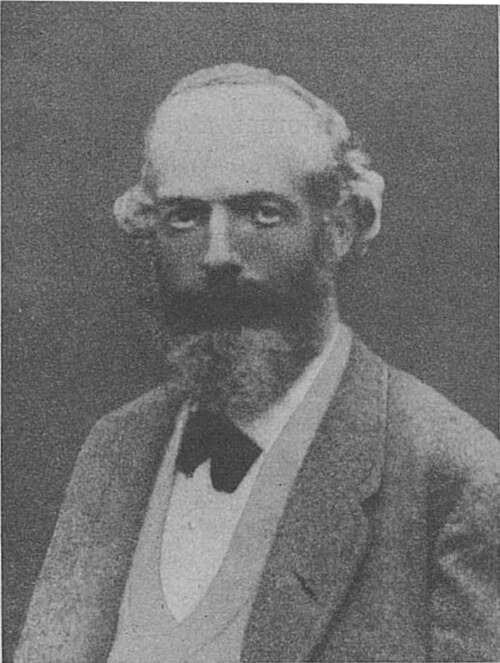
\includegraphics[width=\linewidth]{images/book3/kekule.jpg}
\end{minipage}\hfill
\begin{minipage}[t]{0.74\linewidth}
\vspace{0pt}
Pada tahun 1865 August Kekulé mengusulkan bahwa keenam atom karbon benzena
membentuk cincin dengan ikatan tunggal dan rangkap yang berselang-seling,
dan tak lama kemudian bahwa kedua pola selang-seling itu bertukar begitu
cepat sehingga setiap ikatan sama. Ikatan-ikatan yang sama panjang yang
ditemukan dengan difraksi sinar-X, dan orbital-orbital $\pi$ yang tersebar
di seluruh cincin, memberikan bentuk modern pada intuisinya; \omterm{thm:b2:huckel:huckel-rule}{aturan
Hückel}, pada tahun 1931, menjelaskan mengapa enam elektron, dan bukan empat
atau delapan, membuat cincin istimewa. (Potret, 1873, penulis tidak
diketahui, domain publik, Wikimedia Commons.)
\end{minipage}
\end{history}

\section{Konjugasi dan cahaya}

\begin{proposition}[Celah energi sebuah poliena]\label{prop:b2:huckel:gap}
Dalam poliena linear dengan $n$ karbon ($n$ genap), celah antara tingkat
terisi tertinggi dan tingkat kosong terendah sistem $\pi$ adalah
$4|\beta|\sin(\pi/(2(n + 1)))$: celah itu mengecil ketika rantainya memanjang.
\end{proposition}

\begin{proof}
Tingkat terisi tertinggi adalah $k = n/2$, tingkat kosong terendah
$k = n/2 + 1$. Dengan $\theta_k =
k\pi/(n + 1)$,
$E_{n/2+1} - E_{n/2} = 2|\beta|(\cos\theta_{n/2} - \cos\theta_{n/2+1}) = 4|\beta|
\sin\frac{\theta_{n/2} + \theta_{n/2+1}}{2}\sin\frac{\theta_{n/2+1} - \theta_{n/2}}{2}$,
dan sinus pertama bernilai $\sin(\pi/2) = 1$. Celah itu mengecil seiring $n$
karena $\sin$ naik pada $[0, \pi/2]$.
\end{proof}

\begin{omfigure}
\begin{tikzpicture}
\begin{axis}[width=0.5\linewidth, height=5cm, xmin=0, xmax=22, ymin=0, ymax=2.2,
  axis x line=bottom, axis y line=left, xlabel={jumlah karbon $n$}, ylabel={celah$/|\beta|$},
  tick label style={font=\small}, label style={font=\small}]
\addplot[omThm, thick, mark=*, mark size=1.3pt] table[x=n, y=gap] {figdata/out/bachelor-2-huckel-b.dat};
\end{axis}
\end{tikzpicture}\hfill
\begin{tikzpicture}
\begin{axis}[width=0.48\linewidth, height=5.4cm, xmin=-1, xmax=11, ymin=-2.4, ymax=2.4,
  axis x line=none, axis y line=left, ylabel={$(E - \alpha)/|\beta|$}, clip=false,
  tick label style={font=\small}, label style={font=\small}]
\addplot[only marks, mark=-, mark size=5pt, very thick, omDef] table[x=x, y=e] {figdata/out/bachelor-2-huckel-a.dat};
\draw[densely dotted] (axis cs:-1,0) -- (axis cs:11,0);
\node[anchor=north, font=\scriptsize] at (axis cs:0,-2.45) {C$_2$};
\node[anchor=north, font=\scriptsize] at (axis cs:2,-2.45) {C$_3$};
\node[anchor=north, font=\scriptsize] at (axis cs:4,-2.45) {C$_4$};
\node[anchor=north, font=\scriptsize] at (axis cs:6,-2.45) {C$_6$};
\node[anchor=north, font=\scriptsize] at (axis cs:8,-2.45) {cincin 4};
\node[anchor=north, font=\scriptsize] at (axis cs:10,-2.45) {cincin 6};
\end{axis}
\end{tikzpicture}

{\small Kiri: celah Hückel poliena linear mengecil ketika rantainya
memanjang; itulah sebabnya rantai terkonjugasi yang panjang menyerap pada
panjang gelombang yang lebih panjang, sampai ke daerah tampak. Kanan:
tingkat-tingkat terhitung etena, alil, butadiena, heksatriena (rantai) serta
siklobutadiena dan benzena (cincin); tingkat ikatan berada di bawah
$\alpha$.}
\end{omfigure}

Sebuah heteroatom dimasukkan dengan mengubah \omterm{def:b2:diatomic-mos:integrals}{integral Coulomb-nya},
$\alpha_X = \alpha + h\beta$, dan \omterm{def:b2:diatomic-mos:integrals}{integral resonansi} ikatan-ikatannya: sebuah
model dengan parameter yang dapat disetel, yang mempertahankan hasil-hasil
kualitatifnya (atom elektronegatif, $h > 0$, menarik kerapatan $\pi$ ke arah
dirinya) tetapi yang bilangan-bilangannya dicocokkan, bukan diturunkan.

\section{Latihan}

\begin{exercise}[$\star$]\label{exo:b2:huckel:1}
Berikan $E_\pi$ untuk kation, radikal, dan anion alil.
\end{exercise}

\begin{exercise}[$\star$]\label{exo:b2:huckel:2}
Hitunglah $E_\pi$ butadiena dari tingkat-tingkat $\alpha \pm 1.618\beta$, $\alpha \pm 0.618\beta$.
\end{exercise}

\begin{exercise}[$\star$]\label{exo:b2:huckel:3}
\omterm{def:b2:huckel:aromatic}{Aromatik}, \omterm{def:b2:huckel:aromatic}{antiaromatik}, atau bukan keduanya (jika datar): benzena, anion
siklopentadienil, kation siklopentadienil, kation tropilium \ce{C7H7+},
siklobutadiena, siklooktatetraena datar.
\end{exercise}

\begin{exercise}[$\star$]\label{exo:b2:huckel:4}
Gambarlah lingkaran Frost untuk siklooktatetraena datar dan letakkan kedelapan elektron $\pi$-nya.
\end{exercise}

\begin{exercise}[$\star\star$]\label{exo:b2:huckel:5}
Hitunglah \omterm{def:b2:huckel:delocalisation}{energi delokalisasi} butadiena dan nyatakan dalam \unit{kJ/mol}
dengan $|\beta| = \qty{75}{kJ/mol}$. Bandingkan dengan \qty{10}{kJ/mol} dari
data hidrogenasi sikloheksa-1,3-diena.
\end{exercise}

\begin{exercise}[$\star\star$]\label{exo:b2:huckel:6}
Hitunglah indeks ikatan $\pi$ butadiena dan ramalkan ikatan C--C mana yang
paling pendek.
\end{exercise}

\begin{exercise}[$\star\star$]\label{exo:b2:huckel:7}
Tingkat-tingkat cincin beranggota lima adalah $\alpha + 2\beta$,
$\alpha + 0.618\beta$ (dua kali), $\alpha - 1.618\beta$ (dua kali). Isilah
tingkat-tingkat itu untuk anion dan kation siklopentadienil, lalu
bandingkan.
\end{exercise}

\begin{exercise}[$\star\star$]\label{exo:b2:huckel:8}
Dengan tingkat-tingkat cincin beranggota tujuh, jelaskan mengapa
sikloheptatrienil bromida berperilaku sebagai garam, tropilium bromida.
\end{exercise}

\begin{exercise}[$\star\star$]\label{exo:b2:huckel:9}
Periksalah aturan jejak pada heksatriena, yang tingkat-tingkatnya adalah
$\alpha \pm 1.802\beta$, $\alpha \pm
1.247\beta$, $\alpha \pm 0.445\beta$.
\end{exercise}

\begin{exercise}[$\star\star\star$]\label{exo:b2:huckel:10}
Turunkan tingkat-tingkat heksatriena dari bentuk tertutupnya, serta \omterm{def:b2:huckel:delocalisation}{energi delokalisasinya}.
\end{exercise}

\begin{exercise}[$\star\star\star$]\label{exo:b2:huckel:11}
Siklobutadiena berbentuk bujur sangkar akan mempunyai dua elektron tak
berpasangan. Jelaskan mengapa molekul yang sebenarnya berbentuk persegi
panjang, dengan dua ikatan pendek dan dua ikatan panjang.
\end{exercise}

\begin{exercise}[$\star\star\star$]\label{exo:b2:huckel:12}
Dalam sistem $\pi$ dua atom \ce{C=X} dengan $\alpha_X = \alpha + \beta$ (nilai
model, $h = 1$) dan $\beta_{\ce{CX}} = \beta$, tentukan kedua tingkatnya dan
muatan $\pi$ pada C dan X untuk dua elektron.
\end{exercise}

\section{Soal: Energi Benzena yang Hilang}

\begin{problem}[{Soal akhir pekan --- stabilisasi aromatik benzena dari
entalpi hidrogenasi, tingkat-tingkat Hückel benzena dan energi
delokalisasinya, nilai $|\beta|$, serta perbandingan dengan heksatriena dan
siklooktatetraena}]
\label{pb:b2:huckel:1}
Data: entalpi pembentukan gas-gas (\unit{kJ/mol}): benzena 82.9,
sikloheksa-1,3-diena 104.6, sikloheksena $-4.3$, sikloheksana $-123.1$.
Panjang ikatan (pm): benzena 139.7, etena 133.9, etana 153.6.
% ledger: dfh:C6H6_g, dfh:C6H8_g, dfh:C6H10_g, dfh:C6H12_g, geo:C6H6.rCC, geo:C2H4.rCC, geo:C2H6.rCC

\medskip
\noindent\textbf{Bagian I --- Hidrogenasi.}
\begin{enumerate}
  \item Hitunglah $\Delta_r H^\circ$ hidrogenasi sikloheksena menjadi
        sikloheksana.
  \item Hal yang sama untuk sikloheksa-1,3-diena.
  \item Hal yang sama untuk benzena.
  \item Berapa yang akan dilepaskan oleh tiga ikatan rangkap yang saling
        bebas?
  \item Simpulkan stabilisasi benzena.
  \item Bandingkan dengan stabilisasi diena terkonjugasi, lalu berilah
        komentar.
\end{enumerate}

\medskip
\noindent\textbf{Bagian II --- Benzena menurut Hückel.}
\begin{enumerate}[resume]
  \item Tuliskan matriks Hückel benzena.
  \item Berikan tingkat-tingkatnya dari rumus cincin.
  \item Isilah tingkat-tingkat itu dengan enam elektron $\pi$.
  \item Hitunglah $E_\pi$.
  \item Hitunglah $E_\pi$ tiga ikatan rangkap terisolasi.
  \item Simpulkan \omterm{def:b2:huckel:delocalisation}{energi delokalisasinya}.
  \item Periksalah aturan jejak.
\end{enumerate}

\medskip
\noindent\textbf{Bagian III --- Nilai $|\beta|$.}
\begin{enumerate}[resume]
  \item Samakan \omterm{def:b2:huckel:delocalisation}{energi delokalisasi} dengan stabilisasi pada Bagian I dan
        tentukan $|\beta|$.
  \item Dengan nilai itu, ramalkan \omterm{def:b2:huckel:delocalisation}{energi delokalisasi} butadiena, lalu
        bandingkan dengan Bagian I.
  \item Hitunglah indeks ikatan $\pi$ benzena.
  \item Bandingkan dengan indeks ikatan butadiena.
  \item Jelaskan mengapa panjang ikatan benzena sama dan di mana nilainya
        terletak.
\end{enumerate}

\medskip
\noindent\textbf{Bagian IV --- Cincin dan rantai lain.}
\begin{enumerate}[resume]
  \item Hitunglah \omterm{def:b2:huckel:delocalisation}{energi delokalisasi} heksatriena dan bandingkan dengan
        benzena.
  \item Berikan tingkat-tingkat siklooktatetraena datar.
  \item Isilah dengan delapan elektron: apa yang salah?
  \item Bagaimana molekul yang sebenarnya menghindarinya?
  \item Bagaimana keadaan siklobutadiena?
  \item Nyatakan \omterm{thm:b2:huckel:huckel-rule}{aturan Hückel}.
  \item Nyatakan nilai $|\beta|$ yang diperoleh dengan mencocokkan \omterm{def:b2:huckel:delocalisation}{energi
        delokalisasi} benzena dengan stabilisasinya yang terukur.
\end{enumerate}
\end{problem}
